% !TeX program = pdflatex
\documentclass[aspectratio=169,10pt]{beamer}

\usetheme{Madrid}
\usecolortheme{default}
\setbeamertemplate{navigation symbols}{}
\setbeamertemplate{footline}[frame number]
\setbeamertemplate{caption}[numbered]

\usepackage[T2A]{fontenc}
\usepackage[utf8]{inputenc}
\usepackage[russian]{babel}
\usepackage{amsmath,amssymb}
\usepackage{graphicx}
\usepackage{booktabs}
\usepackage{array}
\usepackage{ragged2e}

\title[Нейросетевые модели уравнения Вебстера]{Разработка физически информированной нейросети для решения уравнения Вебстера}
\author{Г. О. Ерыкалкин \\[0.15em] \normalsize МФТИ, ЛФИ}

\institute{{\normalsize Научный руководитель: \href{https://mipt.ru}{К.\ А.~Беклемышев, МФТИ}}}
\date{Выпускная квалификационная работа, 2026}

\newcommand{\Hdb}{H_{\mathrm{dB}}}
\newcommand{\R}{\mathbb{R}}

\newcommand{\figplaceholder}[2]{%
\begin{center}
\fbox{%
\begin{minipage}[c][#1][c]{0.88\linewidth}
\centering
\vspace{0.15em}
\textbf{Место для рисунка из ВКР}\\[0.3em]
#2
\vspace{0.15em}
\end{minipage}}
\end{center}}

\begin{document}

% 1
\begin{frame}
    \titlepage
    \vspace{-0.5em}
    \begin{center}
        \small 
    \end{center}
\end{frame}

% 2
\begin{frame}{Цель и задачи работы}
\textbf{Цель работы}

\begin{block}{}
Исследовать и сравнить нейросетевые архитектуры для прямой и обратной задач одномерной волноводной акустики на основе уравнения Вебстера.
\end{block}

\vspace{0.5em}
\textbf{Основные задачи}
\begin{itemize}
    \item исследовать нейросетевые модели для аппроксимации отображения ``геометрия -- отклик'';
    \item сравнить архитектуры по точности и скорости расчета;
    \item исследовать подходы к восстановлению геометрического профиля по передаточной функции.
\end{itemize}
\end{frame}

% 3
\begin{frame}{Актуальность}
\textbf{Почему задача важна}

\begin{itemize}
    \item В задачах синтеза речи и моделирования голосового тракта требуется быстро оценивать влияние формы канала на спектральный отклик.
    \item В нефтегазовой отрасли волноводные и трубные модели используются при анализе распространения волн и интерпретации сигналов в каналах и скважинных системах.
    \item Подобные подходы могут быть полезны и для задач поиска дефектов в оптоволокне, где по измеряемому отклику требуется судить о внутренних неоднородностях структуры.
    \item При этом классические численные методы точны, но становятся дорогими при многократных расчетах и в задачах обратного проектирования.
\end{itemize}
\end{frame}

% 4
\begin{frame}{Физико-математическая постановка}
\begin{columns}[T]
\column{0.55\textwidth}
Уравнение Вебстера для давления в канале переменного сечения:
\[
\frac{1}{A(x)}\frac{\partial}{\partial x}\left(A(x)\frac{\partial p}{\partial x}\right)
-
\frac{1}{c^2}\frac{\partial^2p}{\partial t^2}=0.
\]

Передаточная функция волновода определяется как отношение объемной скорости на выходе к объемной скорости на входе:
\[
H(f)=\frac{U(L,f)}{U(0,f)}.
\]

\vspace{0.4em}
Тем самым $H(f)$ характеризует частотный отклик канала. В прямой задаче требуется предсказывать его по геометрии, а в обратной задаче --- по заданному отклику восстанавливать геометрический профиль.

\column{0.40\textwidth}
\begin{center}
    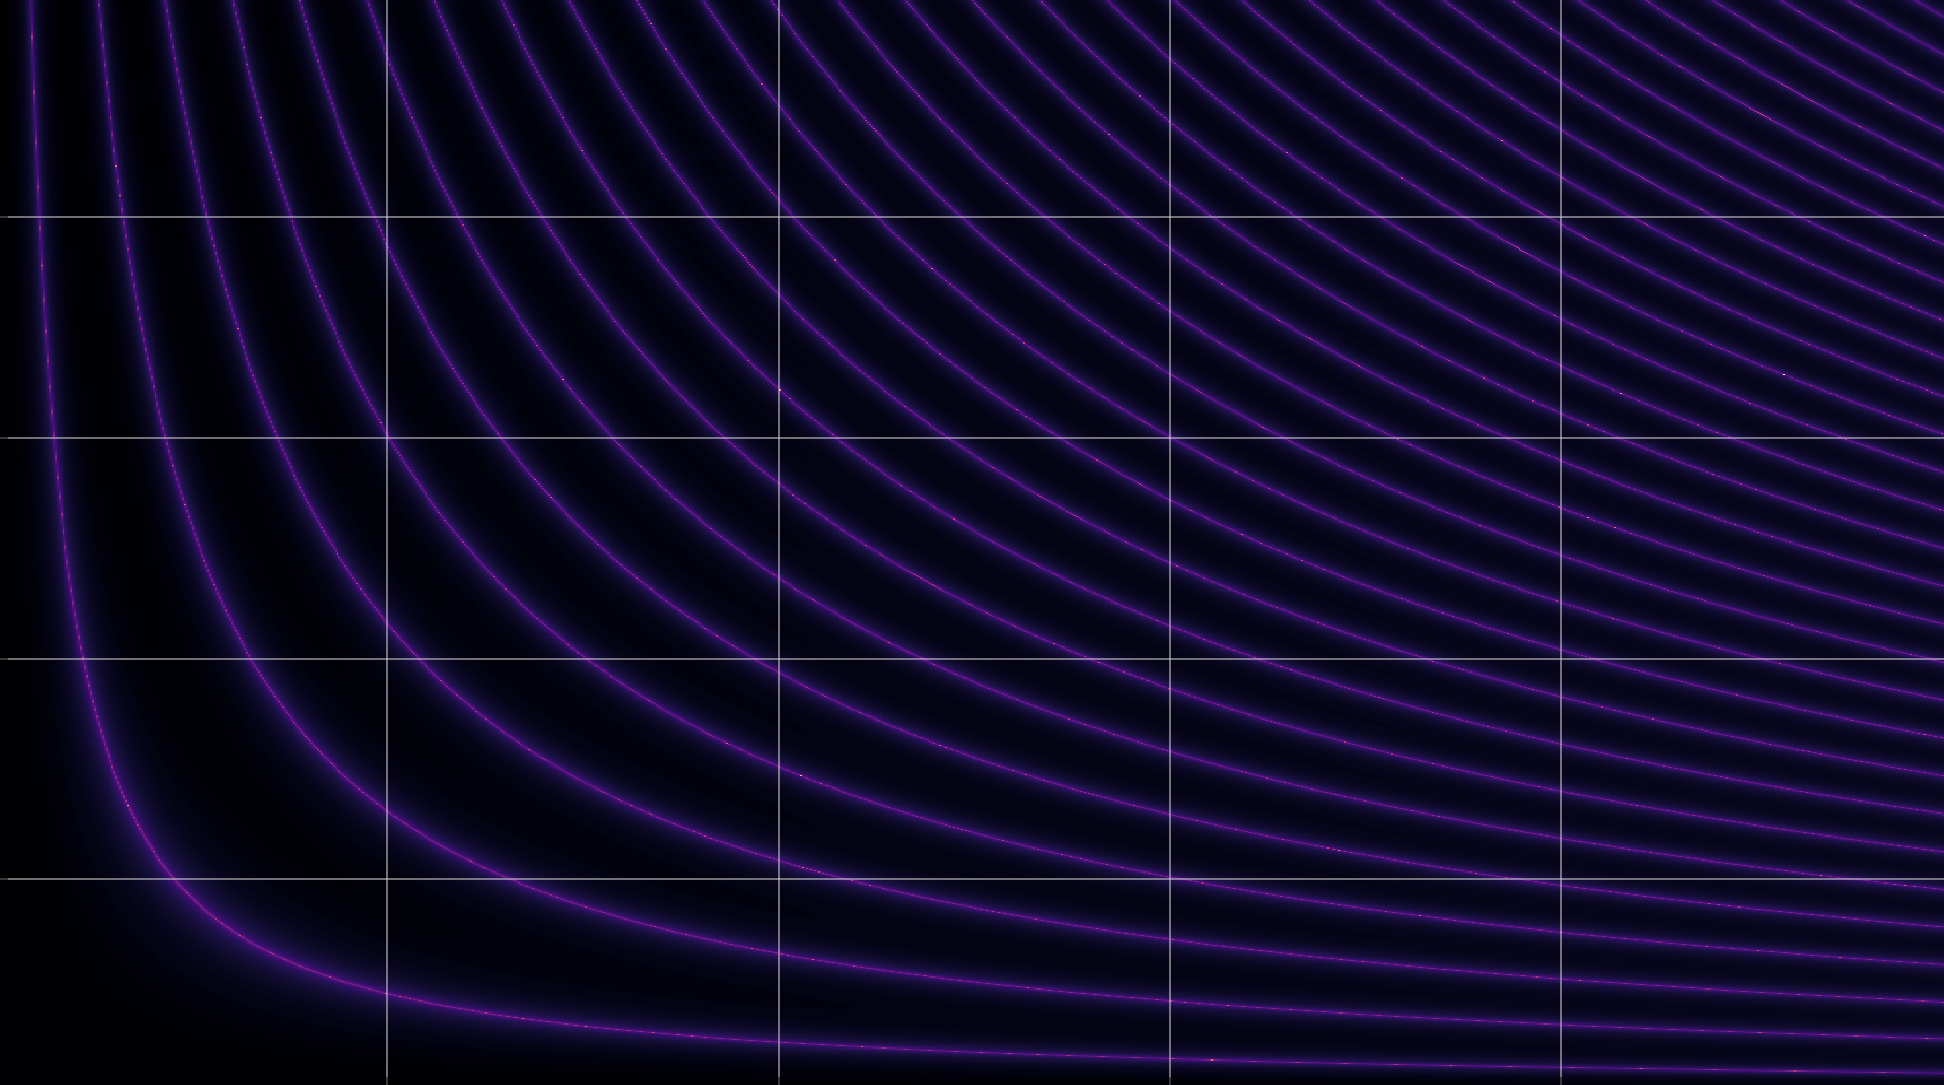
\includegraphics[width=\linewidth]{images/карта.png}
\end{center}
\end{columns}
\end{frame}

% 5
\begin{frame}
\begin{center}
    \Huge Решение прямой задачи
\end{center}
\end{frame}

% 6
\begin{frame}{Постановка прямой задачи}
\begin{columns}[c]
\column{0.40\textwidth}
\begin{center}
    $A(x)$

    \vspace{0.5em}
    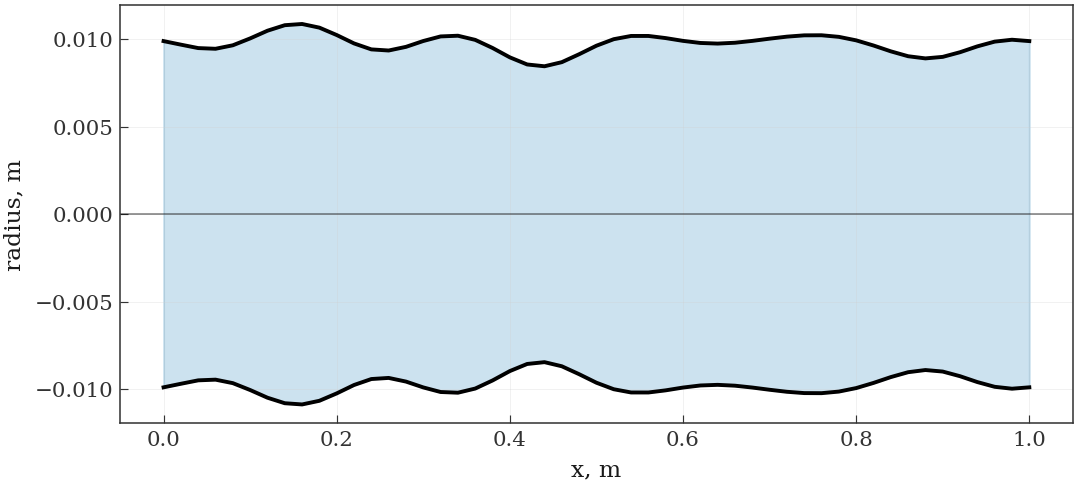
\includegraphics[
        width=0.88\linewidth,
        height=0.50\textheight,
        keepaspectratio
    ]{images/Труба.png}
\end{center}

\column{0.12\textwidth}
\begin{center}
    \Huge $\Longrightarrow$
\end{center}

\column{0.40\textwidth}
\begin{center}
    $H(f)$

    \vspace{0.5em}
    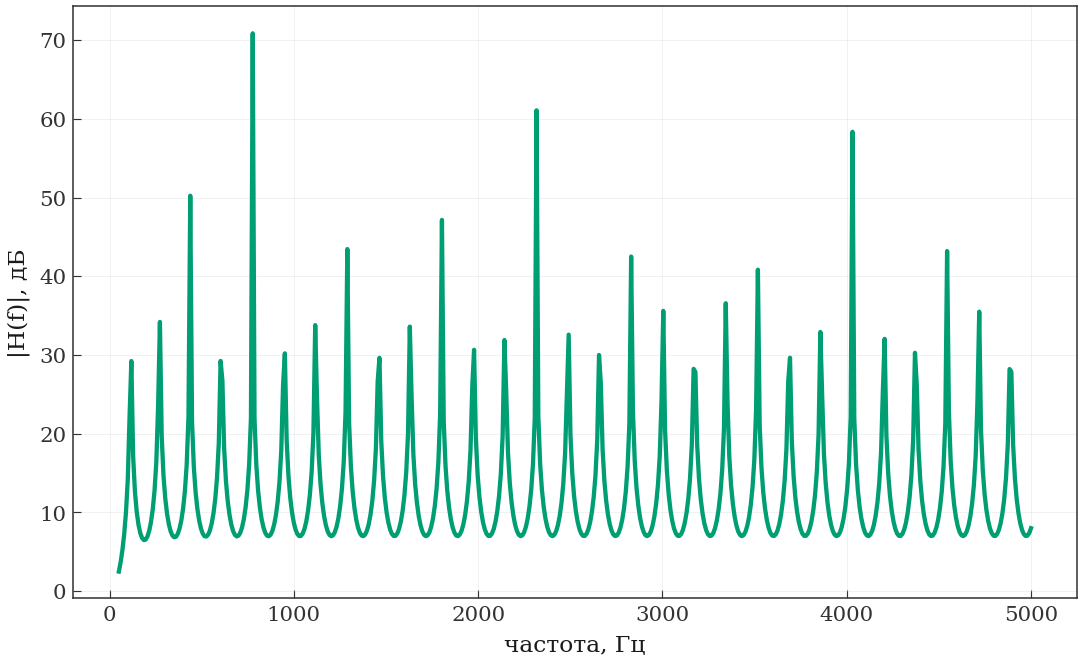
\includegraphics[
        width=0.95\linewidth,
        height=0.40\textheight,
        keepaspectratio
    ]{images/H.png}
\end{center}
\end{columns}
\end{frame}

% 7
\begin{frame}{Методы решения прямой задачи}
\begin{columns}[T]
\column{0.56\textwidth}
\textbf{Численные решатели}
\begin{itemize}
    \item \textbf{Цилиндрический TMM:} канал аппроксимируется последовательностью цилиндрических секций постоянного сечения.
    \item \textbf{Конический TMM:} канал аппроксимируется последовательностью усеченных конусов и точнее описывает плавное изменение радиуса.
    \item \textbf{ARMA-решатель:} использует полиномиальное представление в z-области и позволяет ускорять вычисление спектрального отклика.
\end{itemize}

\vspace{0.4em}
\textbf{Нейросетевые модели}
\begin{itemize}
    \item используются как быстрые суррогаты прямого решателя после обучения;
    \item аппроксимируют отображение ``геометрия канала $\rightarrow$ передаточная функция''.
\end{itemize}

\column{0.40\textwidth}
\begin{center}
    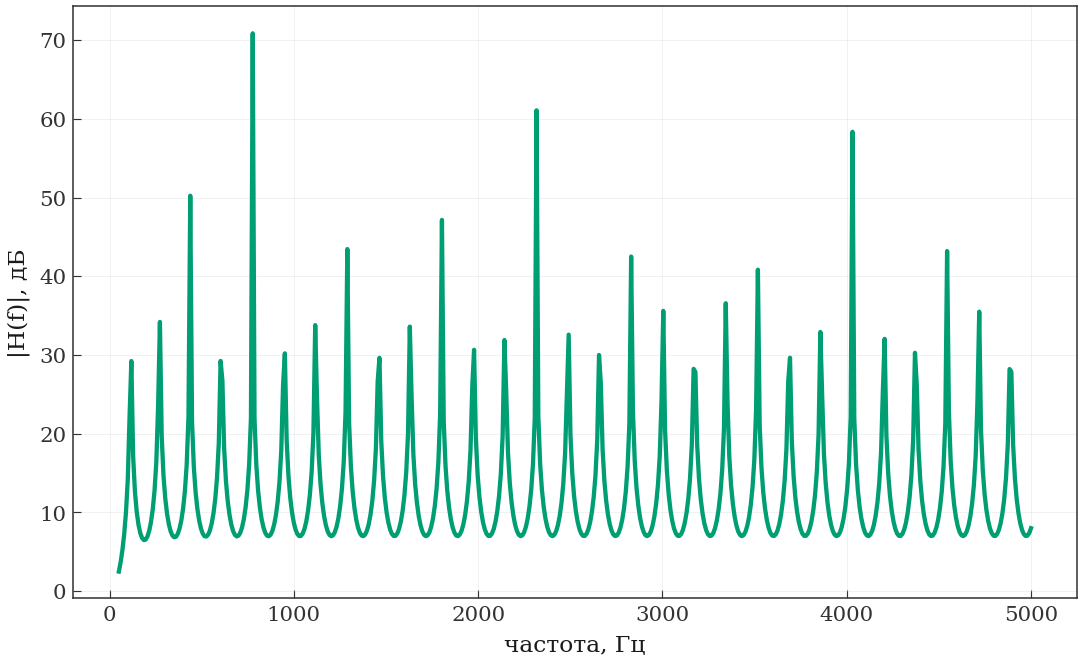
\includegraphics[width=\linewidth]{images/H.png}
\end{center}
\end{columns}
\end{frame}

% 5
\begin{frame}{Данные для обучения}
\begin{columns}[T]
\column{0.48\textwidth}
Для обучения нейросетевых моделей использовались \textbf{синтетические данные}, полученные с помощью численного решения прямой задачи.

\vspace{0.5em}
\textbf{Схема построения датасета}
\begin{itemize}
    \item генерировались различные геометрические профили каналов;
    \item для каждой геометрии численно вычислялась передаточная функция;
    \item пары ``геометрия -- спектральный отклик'' использовались для обучения нейросетей.
\end{itemize}

\column{0.48\textwidth}
\begin{center}
    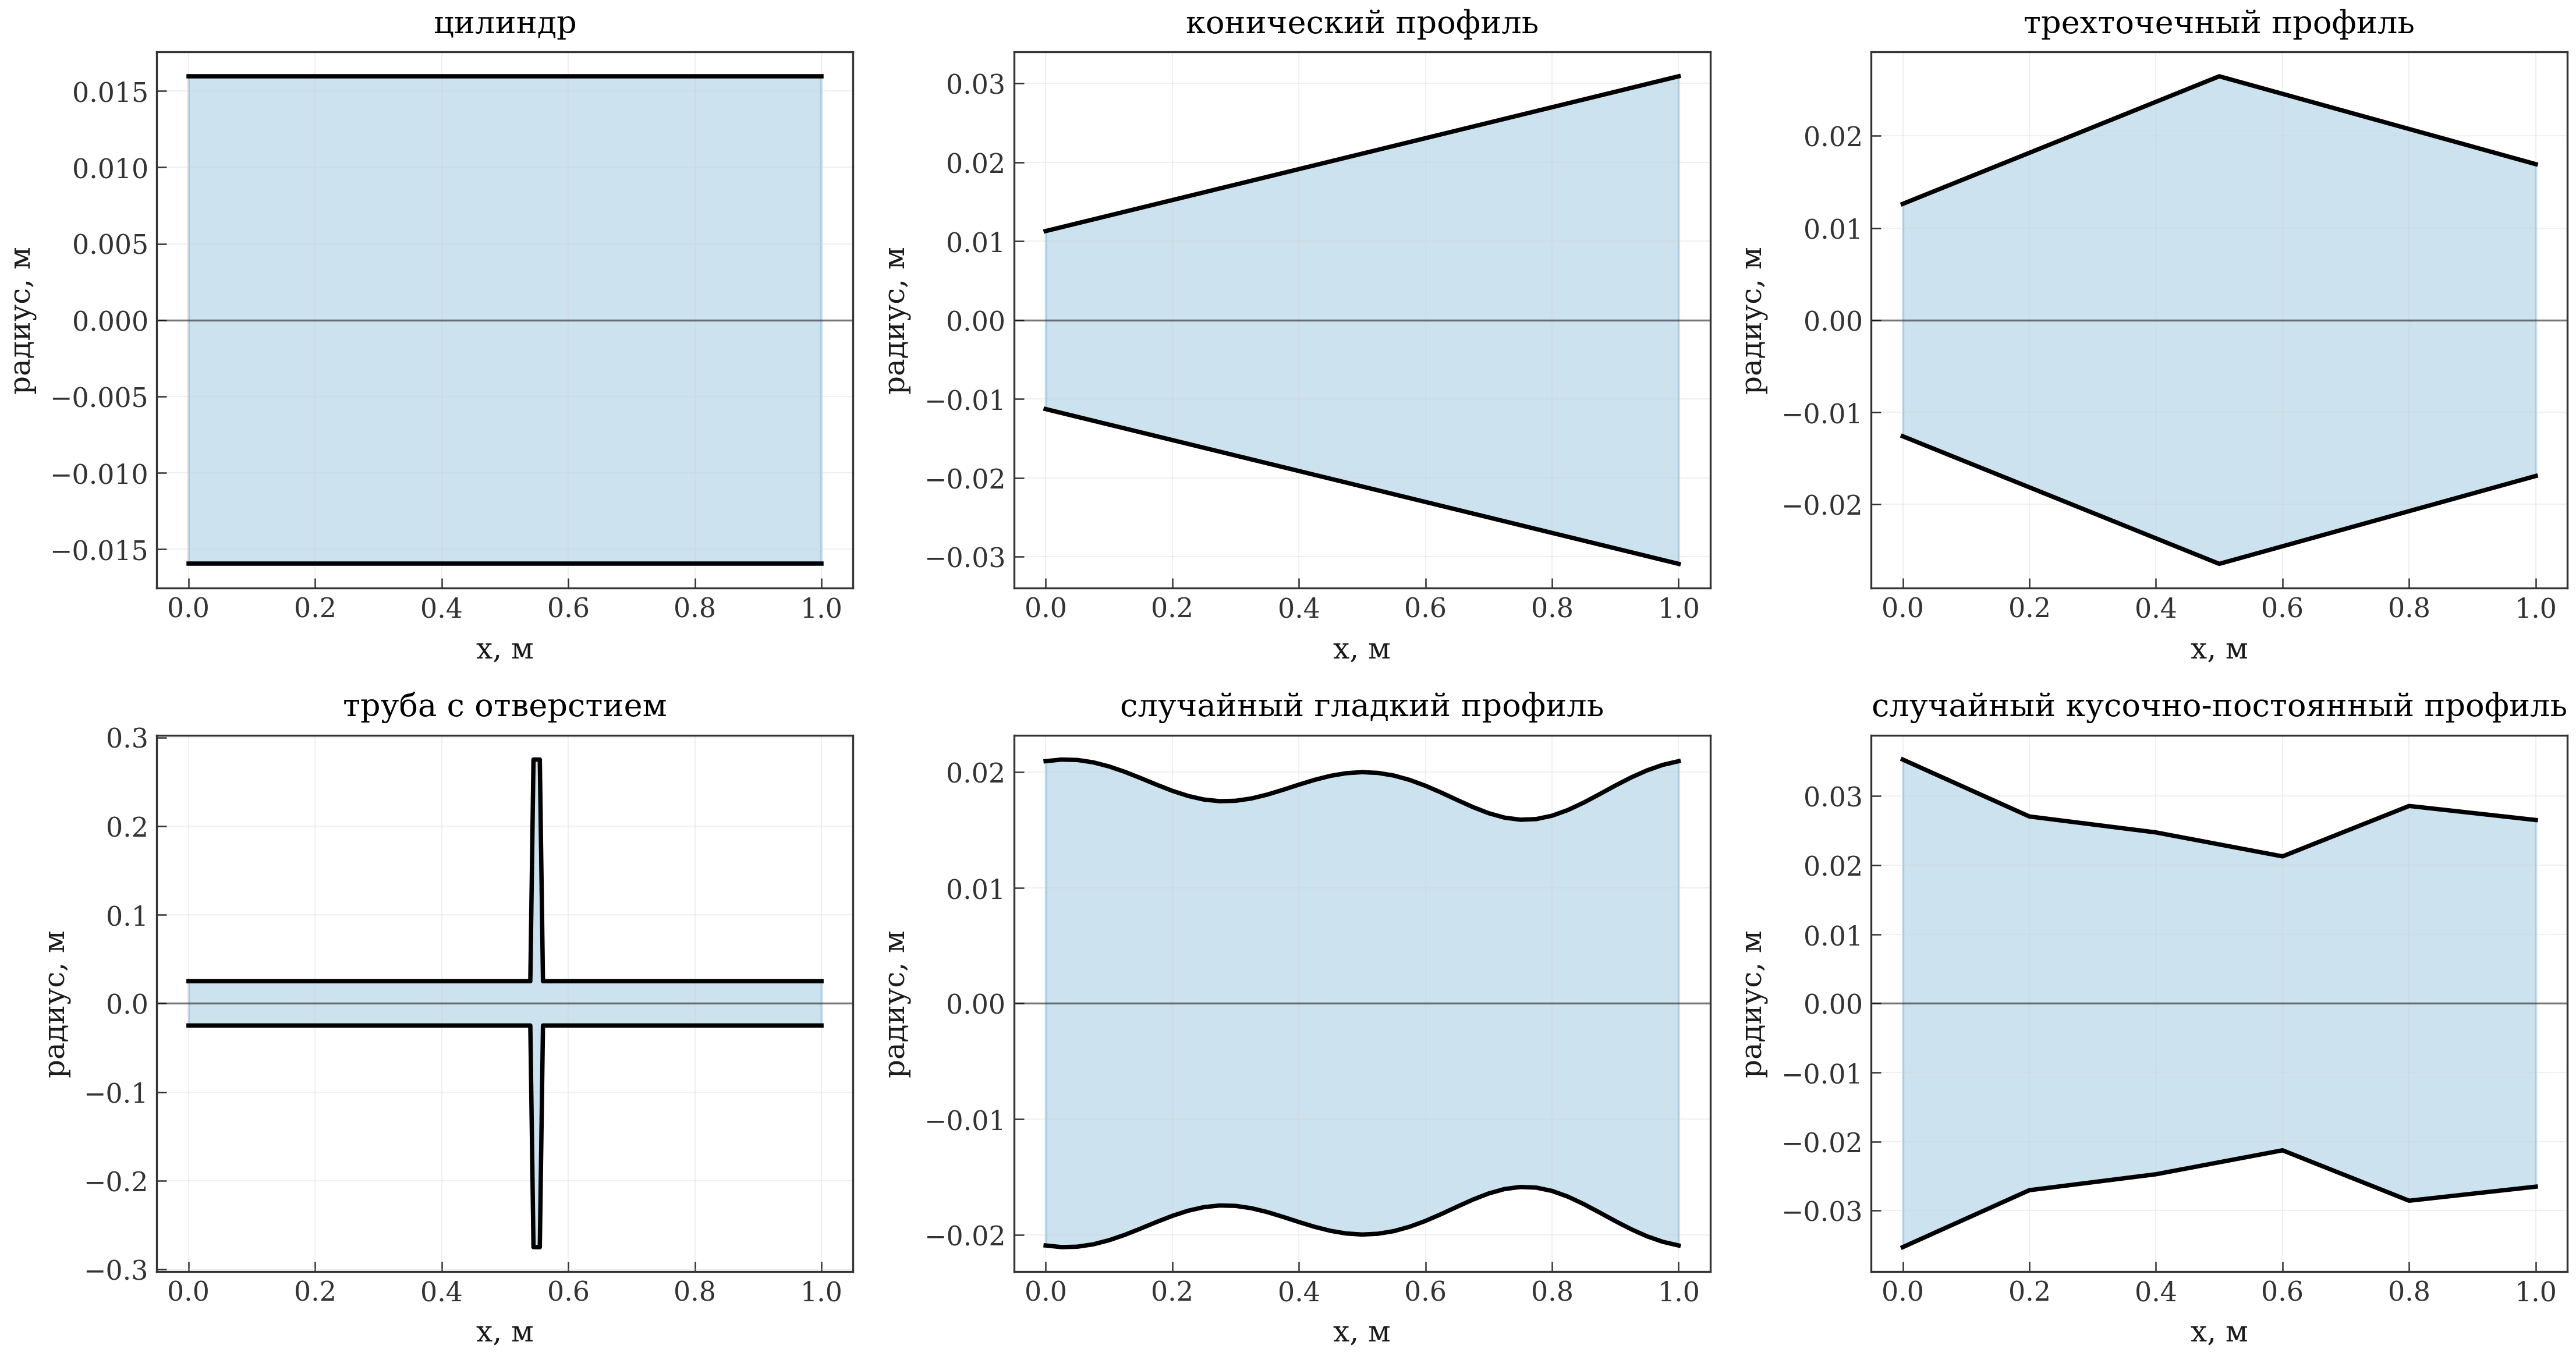
\includegraphics[width=\linewidth]{images/геометрии.png}
\end{center}
\end{columns}
\end{frame}

% 6
\begin{frame}{Прямая задача: постановка для нейросетей}
\textbf{Аппроксимируемый оператор:}
\[
\mathcal{F}_{\theta}: A(x) \longmapsto \Hdb(f).
\]

\vspace{0.6em}
\begin{itemize}
    \item \textbf{MLP} --- базовая полносвязная сеть.
    \item \textbf{CNN} --- сверточные сети.
    \item \textbf{FNO} --- нейронный оператор Фурье.
    \item \textbf{DeepONet} --- нейронный оператор с отдельными ветвями для геометрии и частот.
    \item \textbf{Mamba} --- модель для работы с длинными последовательностями.
\end{itemize}
\end{frame}

% 6
\begin{frame}{Функция потерь и метрики качества}
\textbf{Комбинированный функционал потерь:}
\[
L_{total}=w_{dB}L_{dB}+w_{mag}L_{mag}+w_{deriv}L_{deriv}+w_{peak}L_{peak}+w_{level}L_{level}.
\]

\vspace{0.4em}
\begin{columns}[T]
\column{0.48\textwidth}
\textbf{Что учитывается при обучении}
\begin{itemize}
    \item $L_{dB}$: общее совпадение спектров в дБ;
    \item $L_{mag}$: относительное совпадение линейных амплитуд;
    \item $L_{deriv}$: совпадение формы спектра и его наклонов;
    \item $L_{level}$: совпадение уровней всех найденных пиков целевого спектра.
\end{itemize}

\column{0.48\textwidth}
\textbf{Основные метрики}
\begin{itemize}
    \item MAE, дБ;
    \item ошибка уровня пика, дБ;
    \item ошибка уровня провала, дБ;
    \item относительная ошибка производной.
\end{itemize}
\end{columns}
\end{frame}

% 7
\begin{frame}{Обучение}
\begin{center}
    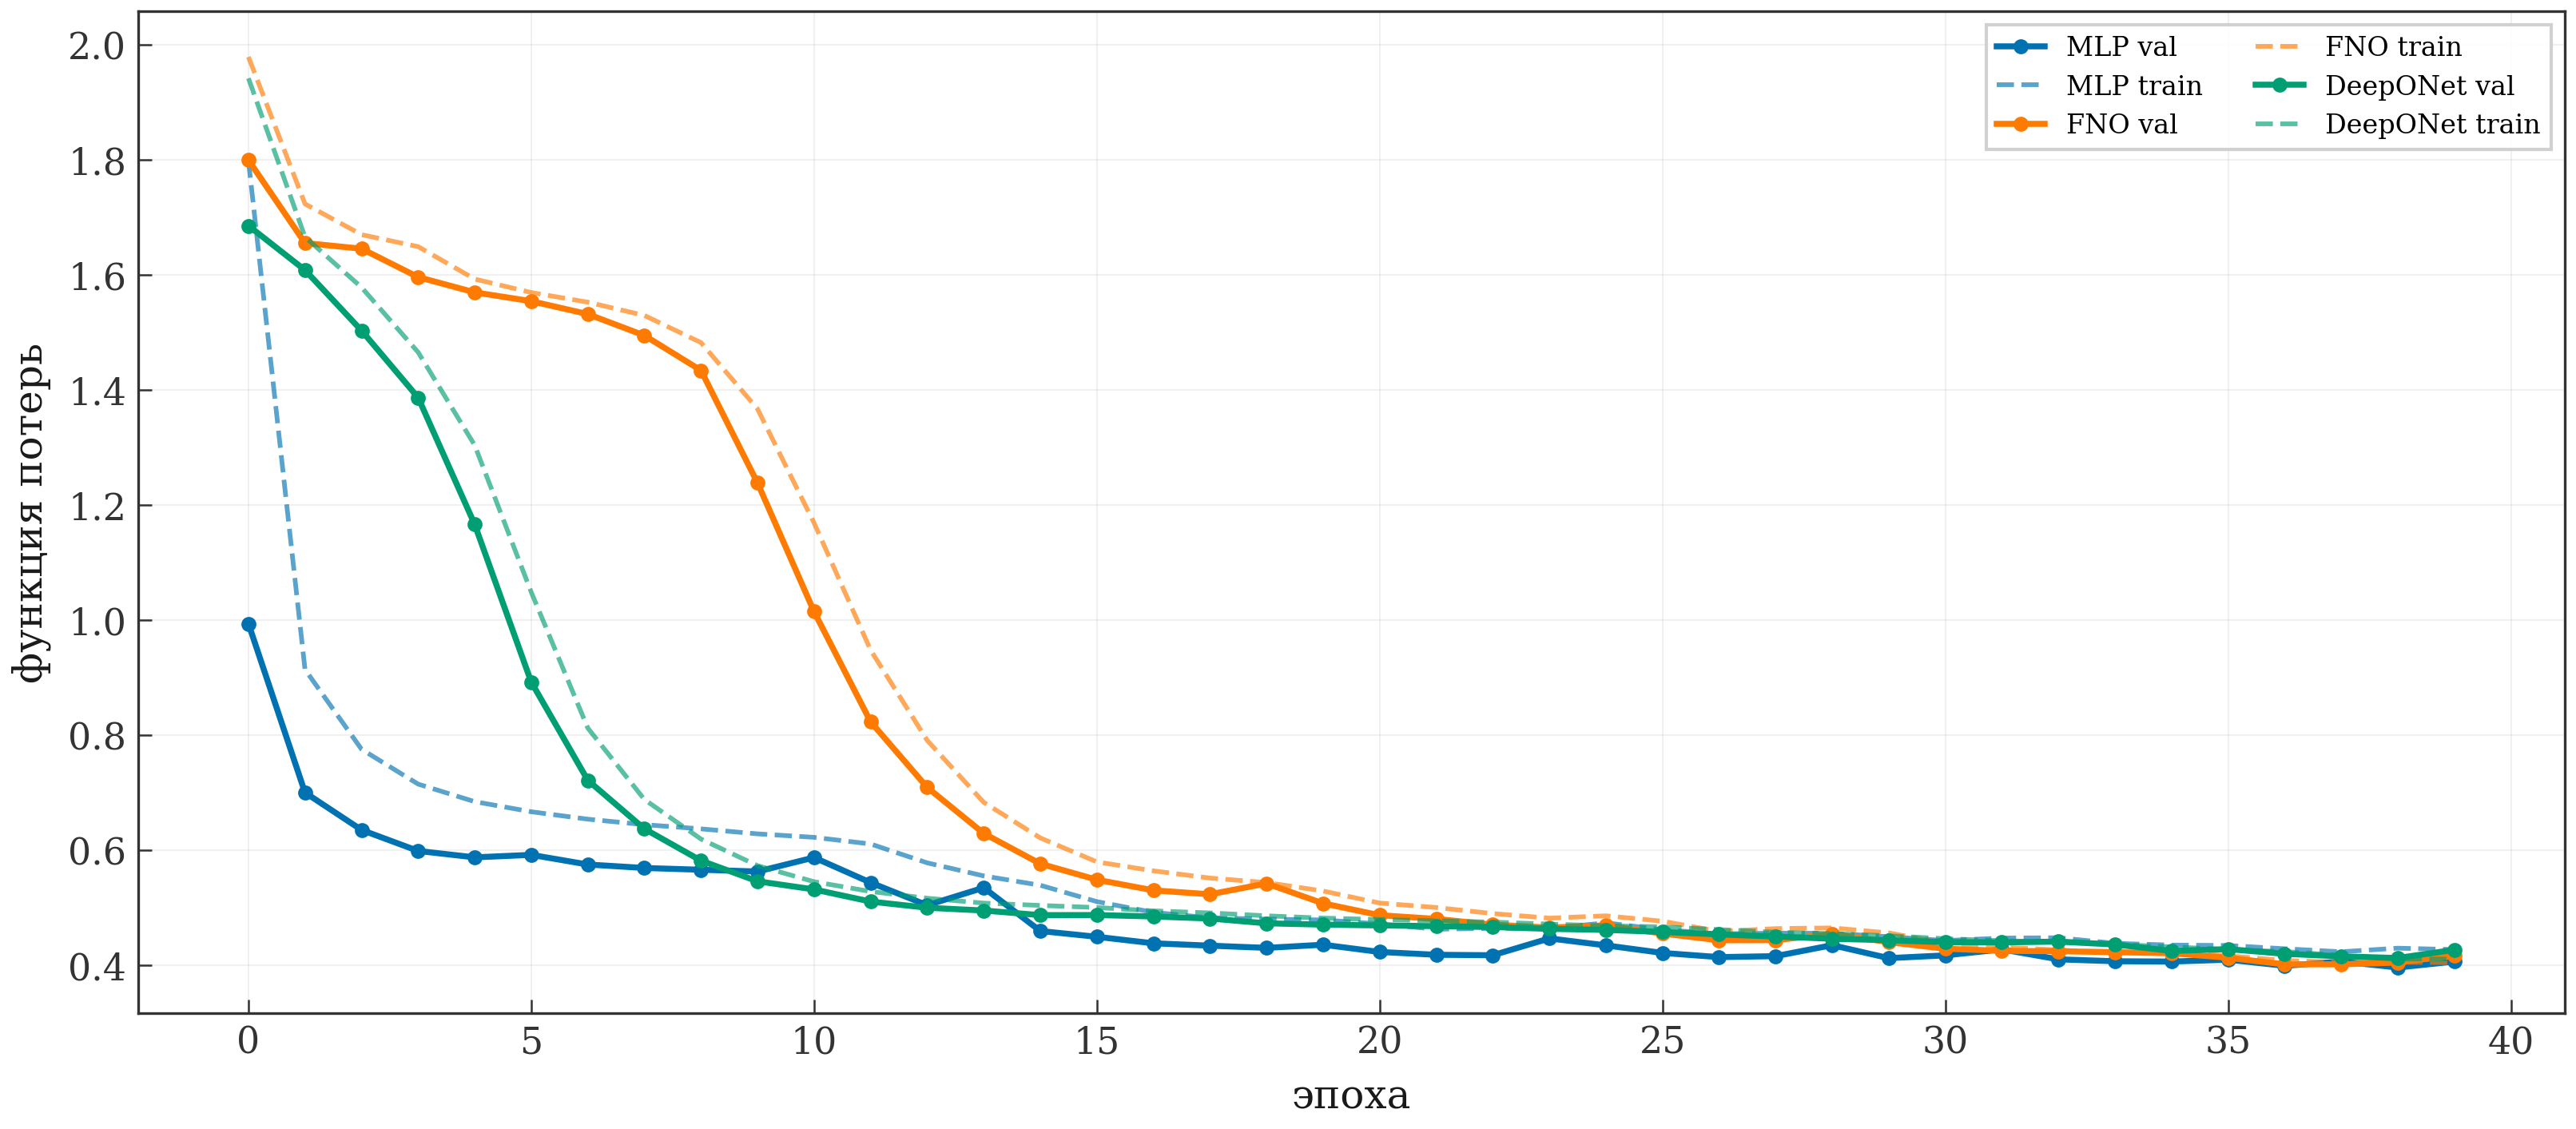
\includegraphics[
        width=0.95\linewidth,
        height=0.78\textheight,
        keepaspectratio
    ]{images/функции_потерь_mlp_fno_deep.png}
\end{center}
\end{frame}

% 8
\begin{frame}{DeepONet: параллельное кодирование геометрии и частот}
\begin{center}
    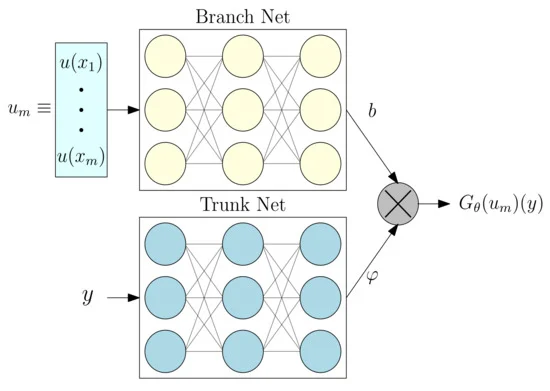
\includegraphics[
        width=0.95\linewidth,
        height=0.78\textheight,
        keepaspectratio
    ]{images/deeponet.png}
\end{center}
\end{frame}

% 9
\begin{frame}{Дополнительное обучение и скорость расчета}
\begin{columns}[T]
\column{0.54\textwidth}
\textbf{70 эпох: Mamba-конфигурации}
\begin{table}
\centering
\scriptsize
\begin{tabular}{lcc}
\toprule
Модель & MAE, дБ & Производная \\
\midrule
Mamba Operator & 1.7041 & 0.4615 \\
Mamba Fusion DeepONet & 1.0016 & 0.3311 \\
\textbf{Mamba SIREN Dynamic Deformable} & \textbf{0.9115} & \textbf{0.3140} \\
\bottomrule
\end{tabular}
\end{table}

\textbf{Интерпретация:} усложненная гибридная архитектура оказалась наиболее эффективной среди Mamba-моделей в отдельном 70-эпоховом сравнении.

\column{0.42\textwidth}
\figplaceholder{0.27\textheight}{Рис. 2.7--2.8: сходимость при 70 эпохах}
\figplaceholder{0.27\textheight}{Рис. 2.9: сравнение скорости нейросетей и решателей}
\end{columns}
\end{frame}

% 10
\begin{frame}{Обратная задача: постановка и оптимизационные методы}
\textbf{Цель:} восстановить профиль $A(x)$ по заданной амплитудной характеристике $\Hdb(f)$.

\vspace{0.5em}
\begin{columns}[T]
\column{0.54\textwidth}
\textbf{Использованные подходы}
\begin{itemize}
    \item градиентная оптимизация через дифференцируемый суррогат;
    \item стохастический поиск по алгоритму Метрополиса;
    \item нейросетевое восстановление с помощью U-Net.
\end{itemize}

\vspace{0.3em}
\textbf{Параметризация оптимизации}
\begin{itemize}
    \item 10 управляющих точек профиля;
    \item сигмоидальные ограничения площади;
    \item регуляризация гладкости и кривизны.
\end{itemize}

\column{0.42\textwidth}
\figplaceholder{0.42\textheight}{Рис. 3.1: сравнение градиентного метода и Метрополиса}
\end{columns}

\vspace{0.3em}
\begin{block}{Наблюдение}
Один пример не доказывает превосходство метода, но показывает чувствительность обратной задачи к параметризации и качеству прямого суррогата.
\end{block}
\end{frame}

% 10
\begin{frame}{U-Net для обратной задачи}
\begin{columns}[T]
\column{0.55\textwidth}
\textbf{Входное представление}
\begin{itemize}
    \item 2D-карта $[H,f,x]$;
    \item режим префиксных откликов;
    \item target: $\log A(x)$.
\end{itemize}

\vspace{0.4em}
\textbf{Итоговая проверка на 100 примерах}
\begin{table}
\centering
\scriptsize
\begin{tabular}{lc}
\toprule
Метрика & Значение \\
\midrule
$\mathrm{MAE}_{\log A}$ & $0.8509 \pm 0.8877$ \\
$\mathrm{MAE}_{H}$, дБ & $4.3630 \pm 1.7952$ \\
\bottomrule
\end{tabular}
\end{table}

\column{0.41\textwidth}
\figplaceholder{0.22\textheight}{Рис. 3.2: карта $[H,f,x]$}
\figplaceholder{0.22\textheight}{Рис. 3.4: примеры восстановления}
\figplaceholder{0.18\textheight}{Рис. 3.5: худший пример и спектральная проверка}
\end{columns}
\end{frame}

% 11
\begin{frame}{Ограничения и интерпретация результатов}
\begin{itemize}
    \item Основной датасет использует фиксированную длину $L=1$ м; для переменной длины требуется отдельный учет масштабирования частоты.
    \item Геометрии с локальной камерой исключены из основной серии, так как оказались трудными для текущих архитектур.
    \item Ошибка уровня пиков остается заметной даже при малой глобальной MAE.
    \item Обратная задача по модулю спектра плохо обусловлена; различие профилей может быть связано как с неоднозначностью, так и с ограничениями оптимизации и суррогата.
    \item Режим префиксных откликов U-Net является исследовательским экспериментом с расширенной информацией, а не постановкой только по одной конечной АЧХ.
\end{itemize}
\end{frame}

% 12
\begin{frame}{Итоги работы}
\begin{enumerate}
    \item Реализован и сопоставлен набор численных решателей уравнения Вебстера.
    \item Сформирован потоковый датасет геометрий и передаточных функций.
    \item Исследованы MLP, FNO, DeepONet, Mamba Operator и модификации DeepONet.
    \item Наилучшее качество в основной серии дала Mamba Fusion DeepONet: MAE $1.0495$ дБ.
    \item В дополнительном 70-эпоховом сравнении лучшей стала Mamba SIREN Dynamic Deformable DeepONet: MAE $0.9115$ дБ.
    \item Нейросетевые модели обеспечивают существенное ускорение прямого расчета.
    \item Для обратной задачи показана сильная зависимость результата от параметризации и входного представления.
\end{enumerate}

\vspace{0.5em}
\begin{center}
\Large Спасибо за внимание!
\end{center}
\end{frame}

\end{document}
